\cleardoublepage
\counterwithout{figure}{section}
\counterwithout{table}{section} 
\counterwithout{equation}{section}
\counterwithin{figure}{chapter}
\counterwithin{table}{chapter} 
\counterwithin{equation}{chapter}


\chapter{Assignment}
\label{sec:aufgabenstellung}
 In frame of this thesis a process is to be developed for generation of the dental color shades using an inkjet printer.  The mechanic aspects of responsible for the movement are not included to the project. A stepper motor driven system responsible for the coordinated movement of the axes controlled by a SmoothieBoard v2-mini is provided by the project partner Bredent GmbH. The specifications of the printing system, like a single drop volume or the max printing distance and angle are to be determined. 
 
 Afterwards, an adequate droplet generator is to be selected. The diameter of the nozzle is as important as the driver technology generating the droplets, which has a direct effect on the optical resolution of the printed pattern. With piezoelectric droplet generators, smaller and faster drops are possible but electromagnetic ones are cheaper. The quantitative coloring behavior depending on the absorption characteristics of the dental ceramic is an unknown to the state of the research and the technology. The shades of the dental colors are to be brought about using the main colors with the highest saturation level and a brightener, which is a water based diluter with  an identical composition to the inks, except lacking the metal-ionic coloring agent. The proportions of the ink and the diluter is not the only parameter affecting the shade of the generated color, but also the application sequence can have a significant effect on the optical perception. Since the translucency of the dental zirconia effects the level of color reflection, the depth of the colored section can have an undeniable effect on the natural look of the dental crown. 
 
 At last, the generated shades are to be verified with the existing color standards. The receipt for each single shade generation has to be prepared. The deployed droplets are not expected to fly and settle on the contact point drying on the surface, but are expected to be absorbed and spread inside the porous material. This nature of the interaction between the ink in its fluid form and porous zirconia defines the system as a nonlinear three dimensional fluid dynamics problem. A model is to be generated taking the every compensational aspect of the nonlinear ink behavior, in order to achieve a point accurate color acquisition.
 
 

\chapter{Expected Advantages and Functions of the Solution}
One of the most important advantages is quantification of the coloring process followed by the printing process. Until this day, the crown coloring process is made by dental technologists all around the world. In other words, all of the dental replacements are partially handcrafted. In the market, hand crafted is another word for made by a craftsman, specifically for the unique owner of the product. Just as any other product on the market, the word handcrafted has a prominent effect on the price tag of the item. The word handcrafted also means the product has some tiny error, a nuance special for each unique sample. If the object of interest is a decor for the home of the consumer, it is one of the most welcome properties. However, if the object of interest is an implant, which is to be carried all the time on the comsumer's body as a part of the it, the property everyone is looking for is perfection. A perfect shape, color, consistency and harmony is a standard to evaluate the quality of the work done by the dentist and of course involving the dental technologist. The quantification of the coloring process is the most important advantage of the solution when it is considered looking from this aspect. Thus, the error can be terminated and the quality deviation can be limited to an acceptable variance. 

Another aspect to consider is the ink costs. Each of the ink bottles are labeled with the same price tag by the manufacturer. However, not all of the ink bottles contain a material worth the same value actually. The shades of the colors ranging from 1 to 3.5 are only diluted versions of the bottle with the shade 4.0. Buying the most concentrated tone and diluting it is here an economical solution, as it is in every other section of the industry. Also, the whole spectrum of shades can be obtained with only 4 ink bottles and a brightener by halftone printing. The required purchase variety, transportation costs, and the space requirement are all reduced with the usage of only the most saturated shades.

\chapter{Solution Structure}
The structural concept is based on the utilization of a 5-axis printing system. A basic microcontroller designed for the automation of the router systems is connected to stepper motors and encoders to control the coordinated printing processes. 4 base colors with the highest saturation levels (A, B, C and D4) are to be used with the brightener to color the dental zirconia, instead of 17 bottles consisting of 16 predefined shades plus the brightener. The amount of the brightener defines the shade of the color. Therefore, the space requirement of the machine is reduced. The inks and the brightener are continuously fed into a rotary distribution valve and are in their neutral status not flowing in any direction. As soon as the rotary valve opens the gate of any incoming pipe,the flow is permitted to the droplet ejector.  
\newline
\begin{figure}[h]
	\centering
	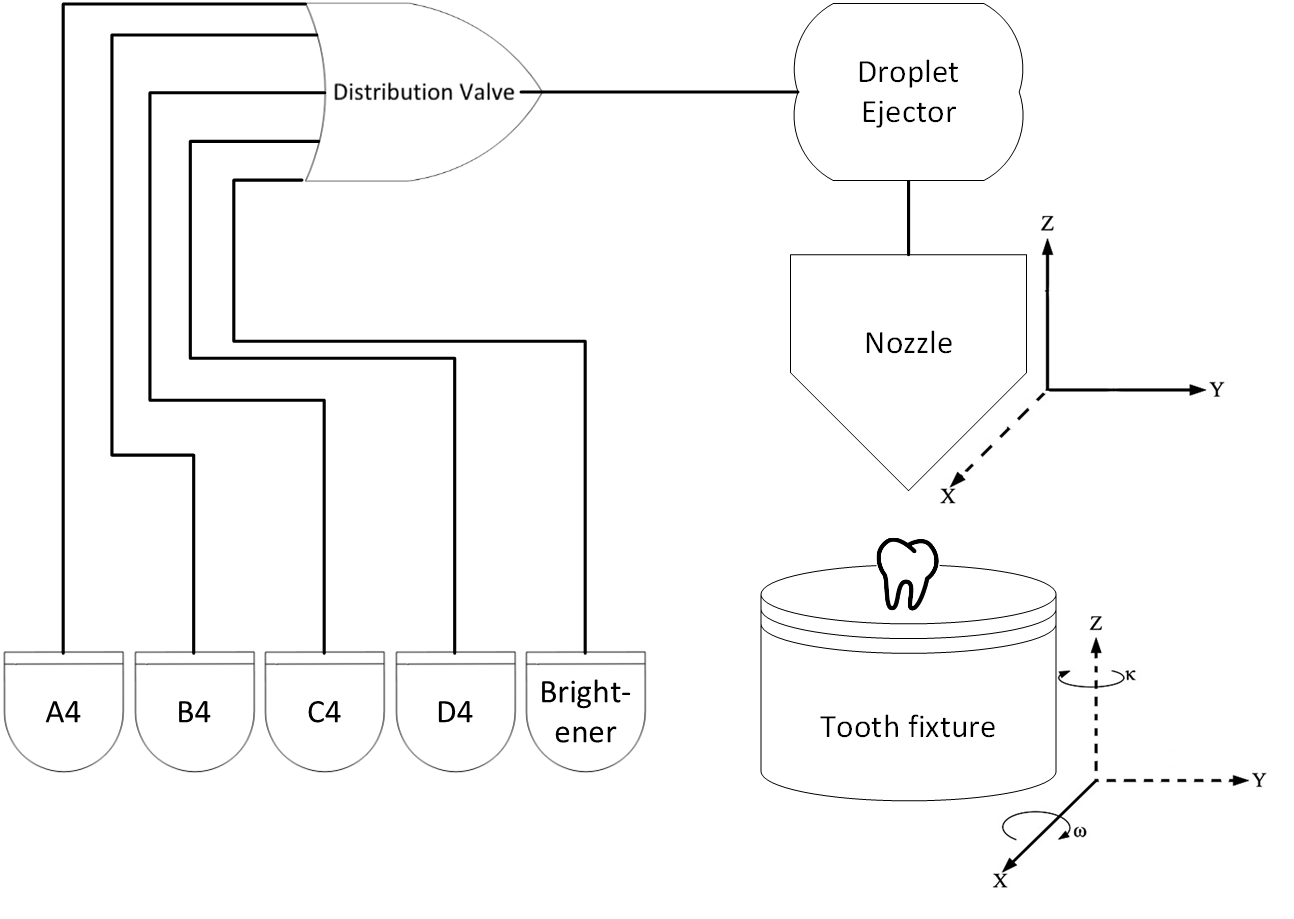
\includegraphics[width=0.9\textwidth]{grafiken/SolutionStructure.jpg}
	\caption{Solution Structure}
	\label{fig:SolutionStructure}
\end{figure} 
\newline
A serial communication between the controller and the rotary valve arranges the position of the rotary valve and the duration to hold on in that position. The required mixture is dosed and pulled by the droplet ejector and deployed through the nozzle, driven by the pressure difference between the ink bottles at the beginning of the cycle and the atmosphere. A 3-axis table and the 2-axis nozzle holder are responsible for the coordination of the flying drops and the point on the surface of the dental crown where the drops need to land during the printing process.

\chapter{Solution Processes}
\label{sec:Lösungsprozesse}
The process concept is realized in three stages. Each stage depends on the previous one and cannot be proceeded to, before the previous one is completed.

\bigskip
\begin{figure}[h]
	\centering
	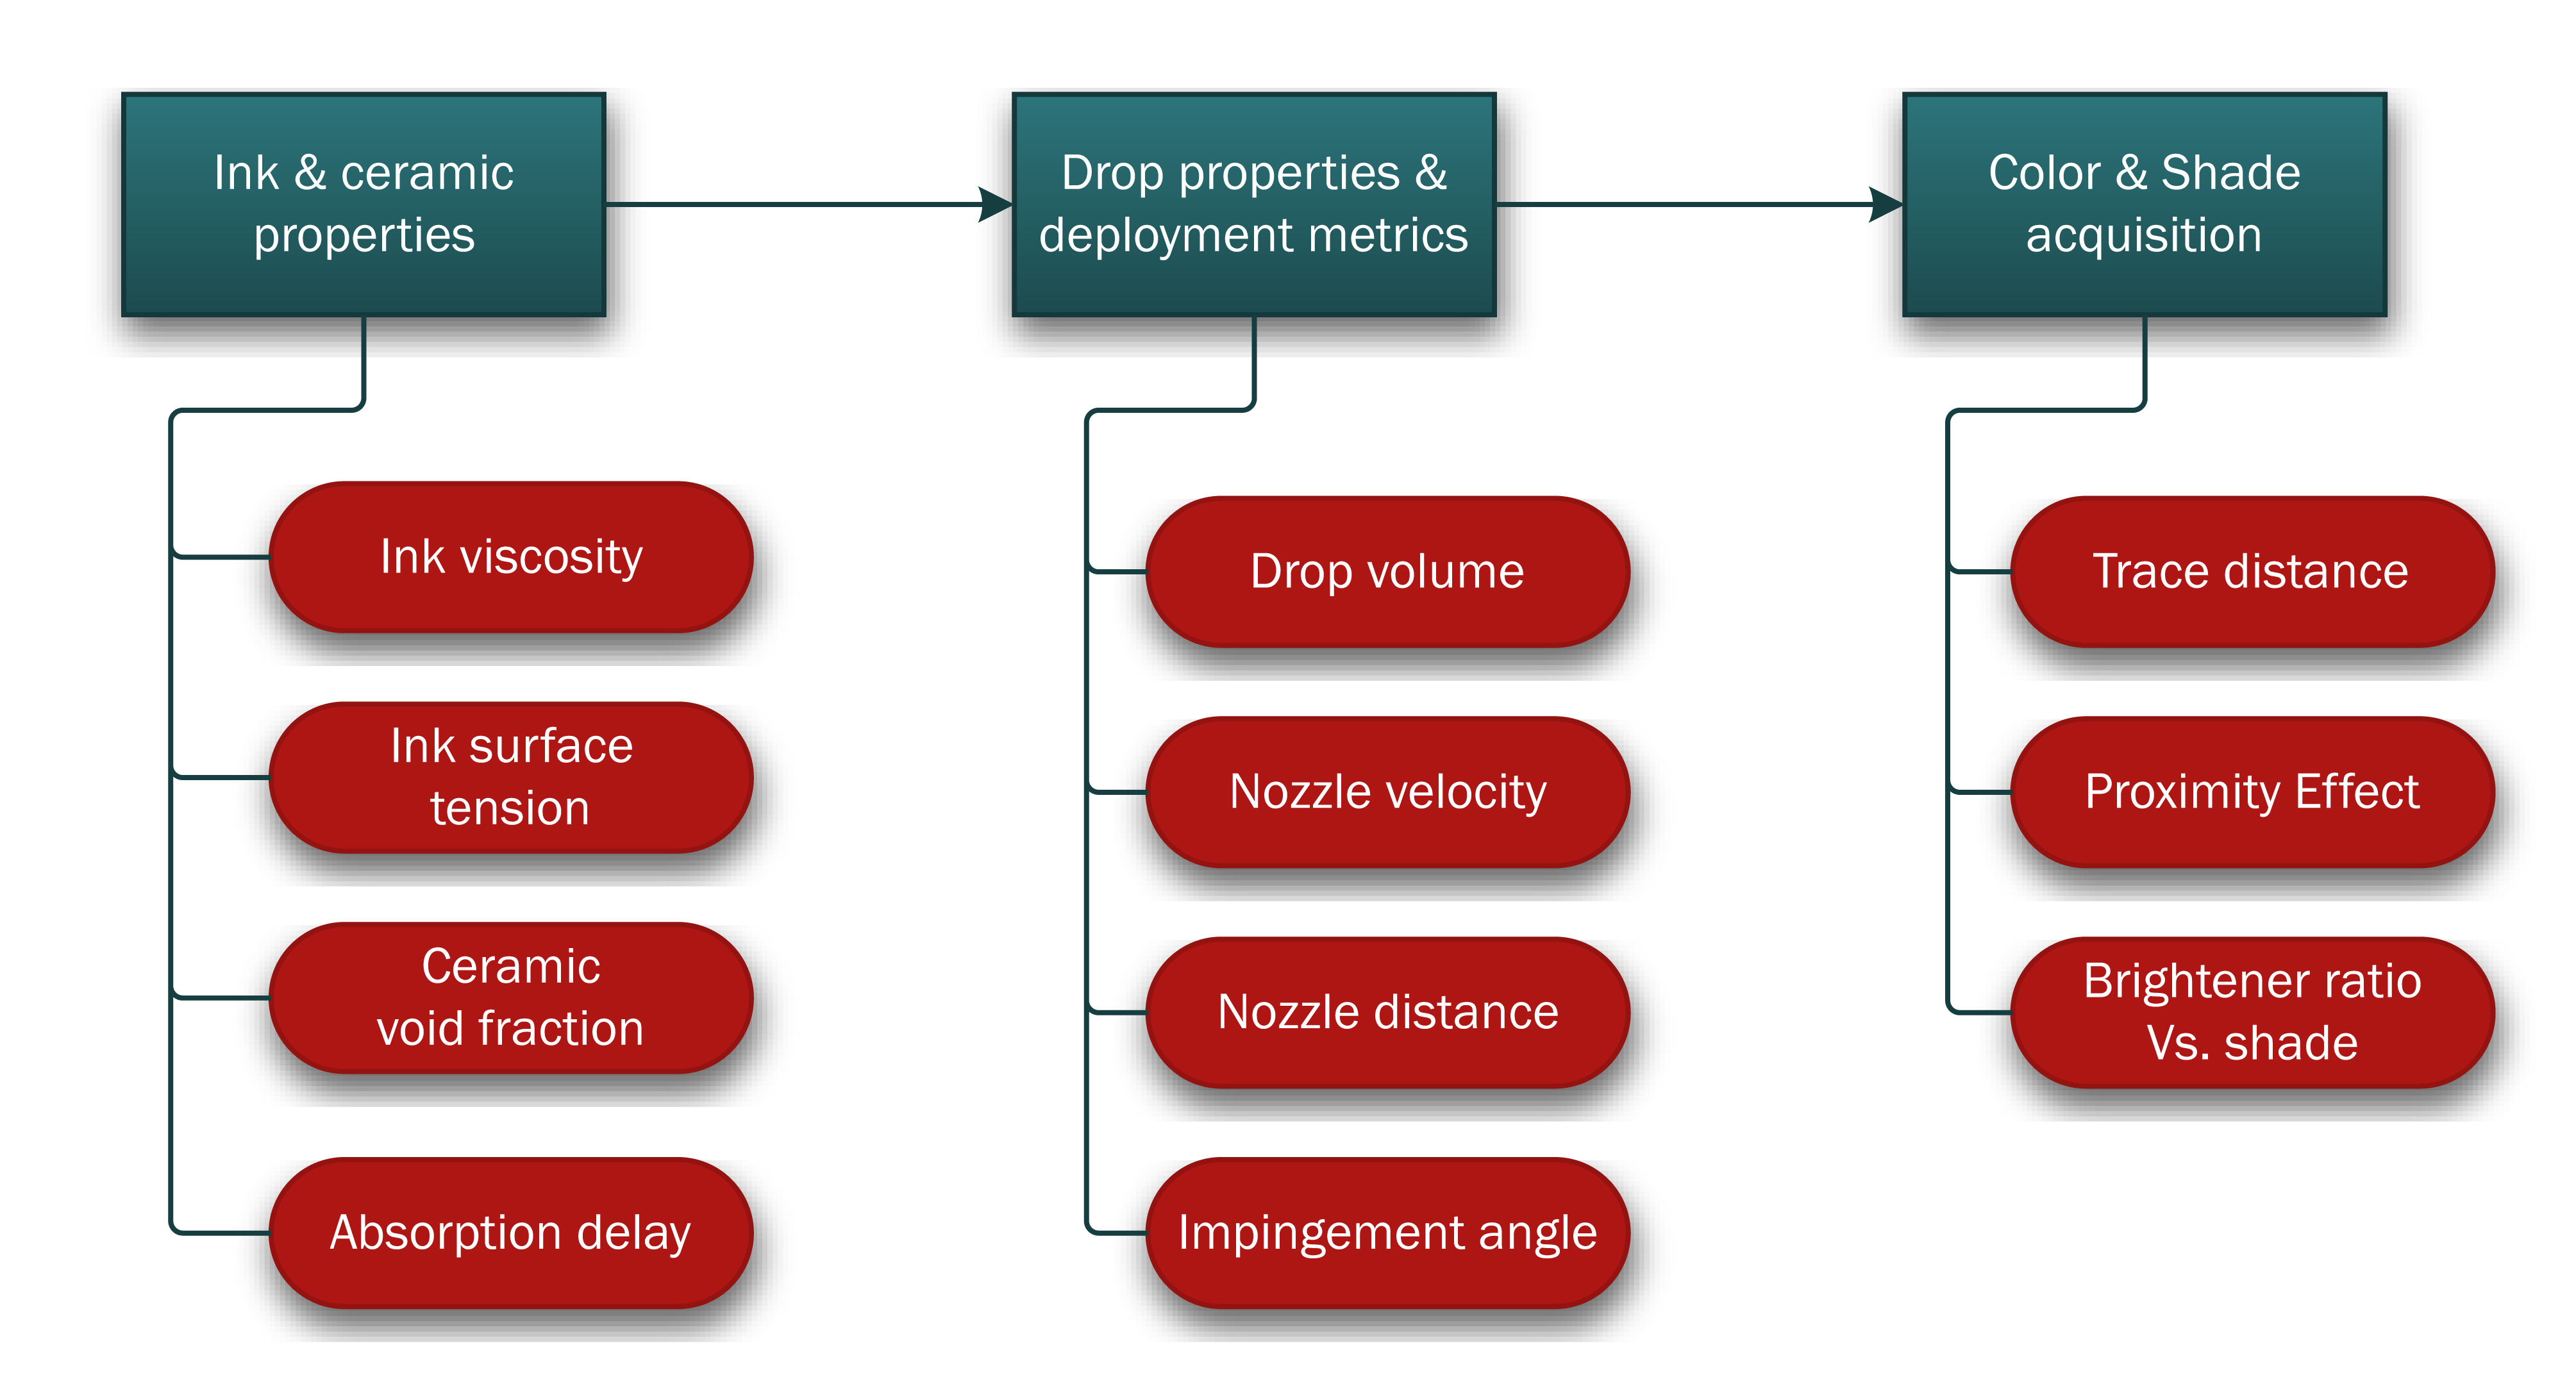
\includegraphics[width=0.9\textwidth]{grafiken/SolutionProcesses.jpg}
	\caption{Solution Processes}
	\label{fig:SolutionProcesses}
\end{figure} 
\bigskip


 First stage is finding the ink and ceramic properties, such as ink viscosity and surface tension, ceramic void fraction and ink absorption time. Depending on these experimentally acquired parameters the equations \ref{eq:InfTime} and \ref{eq:SpreadingDia} can be utilized  in the progress of the model generation for the drop deployment algorithm for an arbitrary pattern to be printed on the zirconia material. 
 
 Second stage is planned to help determine the parameters defining the printing system. It basically focuses on the settlement of drop properties and deployment metrics, which consist of drop volume, nozzle escape velocity of the drops, the optimal distance between the nozzle and zirconia surface and the angle between the drop projectile and the surface. The drop volume has to be determined as soon as possible, because it directly affects the selection of the actuator which is to be used as the drop ejector. Selection of a larger drop size means a shorter printing time. However it also means that the resolution is supposed to become lower. Due to the absorption characteristics of the zirconia material, a critical drop size is expected to cause a significant effect on the diameter of a painted spot. In other words, deploying the same amount of ink on the same spot using drops with a volume of smaller than 5 nL could give the same printed spot diameter.In comparison to the aforementioned drop volumes, using  10 or 20 nL drops to apply the same amount of ink on a single point could result with an unexpectedly larger spot size with lower central intensity. This critical drop size has to be determined, in order to proceed to the rest of the experiments.  
 
 The projectile velocity of the drops is one of the most important parameters affecting the printing system on a temporal basis and also the spreading characteristics of the ink within the porous medium. It is known that for Weber numbers higher than 50, the drops are expected to splash upon the impact with the surface \citep{clarke2002spreading}.
 
 \bigskip
 \begin{equation}\label{eq:weber}
 We=\frac{\rho rv^2}{\gamma}
 \end{equation}
 \bigskip
 
 The maximum distance of the nozzle to the zirconia surface has to be limited. The projectile of the droplets are not perfectly identical. There is a deviation of the impact point, because of the factors like a slight change of the nozzle escape angle of an arbitrary droplet or drag caused by the spontaneous fluctuation of the air flow inside the printing chamber. The longer the fly distance of the droplets are, the less accurately they will meet the same point. So the deployment distance for the droplets should be as short as possible. However on the otherside the geometri of the crown creates the second boundary of the problematic. The concave structures on the upper side of the teeth carrying out the chewing function pose a collision danger with the nozzle. This is a situation where the printing angle is also influential. 
 
 The aspects to be considered under the third stage are employed to conduct an experimental approach to color and shade acquisition. In order to arrive there some parameters have to be determined. Firstly the appropriate trace distance for the selected drop size is to be concluded, depending on the experiment with varying trace distances, which is the distance between two sequential lines on the printed surface. The proximity effect is the second nonlinear parameter affecting the print resolution and color distribution, which refers to how the proximity of two colored areas affect the shade of the uncolored area in between.Finally the dependency of the shade on the brightener ratio is to be determined. For a liquid inside a bottle it is very easy to come to a final conclusion. However, the porous translucent medium has a huge influence on the perceived shade, because of the  reflections form various depths of the material and photons following diverse paths through the sintered zirconia to the eye of the observer.
 
 All of the aforementioned tasks are to be carried out so at the end a model can be generated. This model has to work as an algorithm to calculate the input pattern for a desired arbitrary shade map of a dental crown geometry. The coloring behavior on the printed sample has to be compared with the virtually printed geometrical model.
 

\chapter{Distinctive Features of the Solution}
\label{sec:Unterscheidungsmerkmale}
The most contemporary dental laboratory of today still has to do the coloring process manually. A dental technologist uses brushes to apply tens of bottles of ink shades to the dental crowns one by one following the procedures described by dental zirconia ink manufacturers. Coloring each tooth takes about 5 minutes and about 100 precise brush strokes. This is a process which requires a high patience and repeatability. This project is the first automated printing approach in dental coloring sector. With the automation of the procedure many advantages are expected. The accuracy of shade acquisition is to be guaranteed because of the quantified and digitalized coloring procedure. The variation between the sequential teeth are to be minimized. Shorter lead times can be realized upon the optimization of the printing method, which is to be accompanied by lower costs due to the automation and shortened process time.

Another novelty of the project is the discontinuation of the requirement for a bottle for every single shade of each color. The lighter shade of each color are only bottle mixtures of the brightening fluid and the darkest shade of that color by the manufacturer. The mixtures do not posses a linear ratio for the contained ink and brightener depending on the color shade. The mixture is prepared considering the end shade to be acquired on the zirconia. This project makes it possible for the first time to generate the shades using the darkest base colors and a brightener, thanks to the digitalization of the coloring procedure.

\chapter{Experiments}

Before moving on to the experiments I want to show you the 5 axis printing system prototype provided by Bredent for conduction of the experiments. 
It utilizes a single nozzle print head  with a piezoelectric valve to generate the droplets. Ink selection, positioning and drop generation commands are given with a G-Code.
\begin{figure}[h]
	\centering
	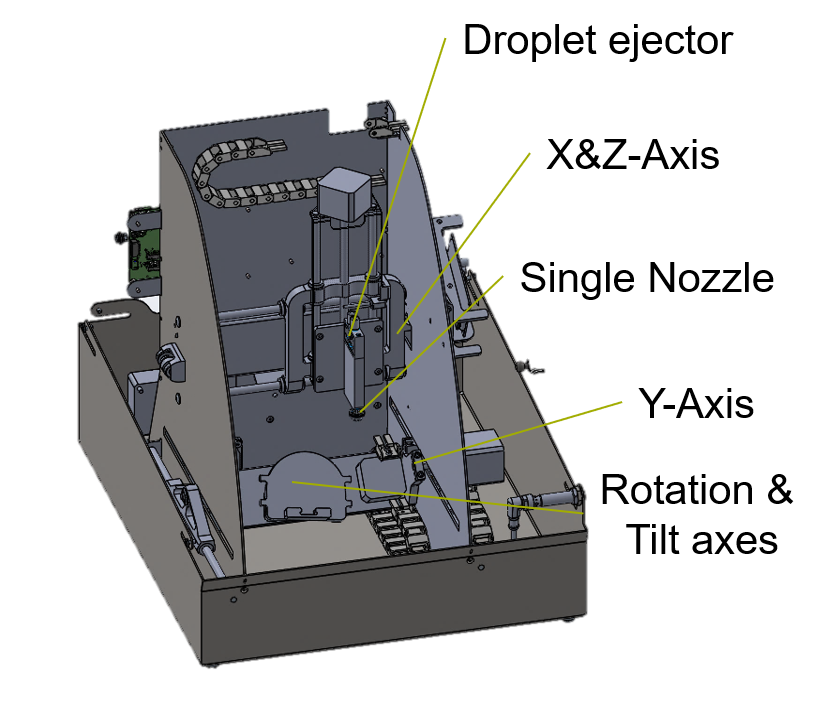
\includegraphics[width=0.7\textwidth]{grafiken/PrototypeText.png}
	\caption{5 axis printer design for dental ink (Matthias Leininger, Bredent GmbH)}
	\label{fig:Prototype}
\end{figure} 

\section{Material Properties}
For a dental technician it is totally trivial how viscous the ink is but for an automated printing  process the quantization of the properties is highly important. In the first experiment, the properties of the coloring agents A1, A2 and A3.5 are determined and compared to those of water. The inks have a similar density to water, but with increasing coloring agent the surface tension gets lower and the viscosity gets 3 times higher when compared to water.Also, a porosity measurement for the zirconia is conducted, which revealed a 43 percent void fraction. The raw volumetric porosity measurements are 43.09,	43.00 and 43.70. The consistency of the results is also a sign for randomly close packed zirconia powder during the manufacturing procedure. Otherwise the irregular packing would inhibit the fluid drainage and cause macro voids inside the porous material after the dissipation of the impregnating liquid, which would also lead to porosity measurements with a significantly large standard deviation. 
 
\begin{figure}[h]
	\centering
	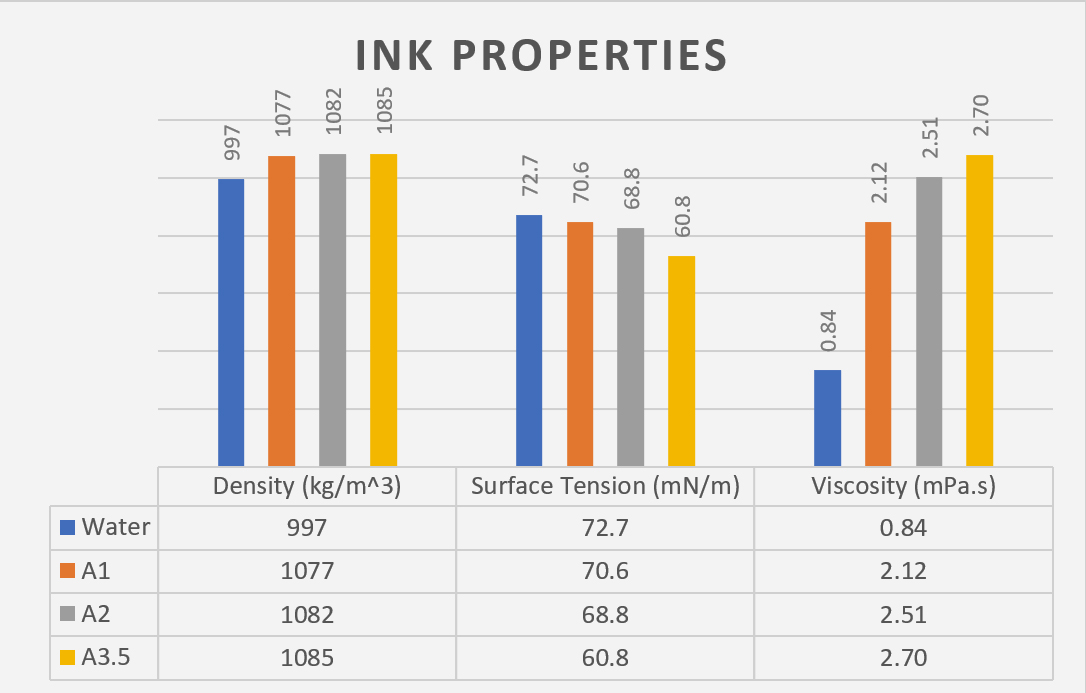
\includegraphics[width=0.8\textwidth]{grafiken/InkProps.jpg}
	\caption{Ink Properties}
	\label{fig:InkProps}
\end{figure} 

\section{Absorption Time}
The second experiment is about the absorption time of the droplets which limits the printing time. We wanted to see whether a heat source can accelerate the absorption or not.
The Absorption times are measured at temperatures ranging from 20 to 80 deg cels.The results show that a change of 60 degrees provide a 50\% reduction in time.

\begin{figure}[h]
	\centering
	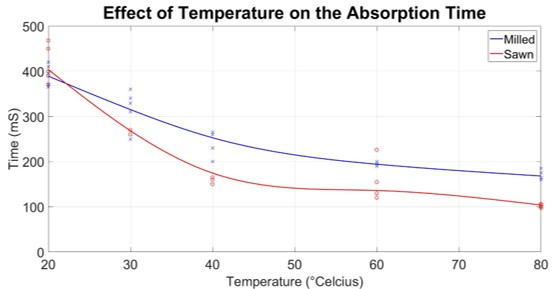
\includegraphics[width=0.8\textwidth]{grafiken/AbsorptionTime.jpg}
	\caption{Effect of heat on the absorption time}
	\label{fig:AbsorptionTime}
\end{figure} 

\section{Drop Size Selection}
The purpose of the third experiment is deciding for an adequate drop size. Depending on the drop size the drop generator is to be selected. In this figure you can see a printed zirconia specimen. Each spot on the upper half has a total ink volume of 800 nL and the ones on the bottom half 400 nL. These spots are printed using drops with volumes of 100, 50, 25 and 12.5 nL.The first image shows the spots right after printing. The second one shows the surface after furnacing.
\begin{figure}[h]
	\centering
	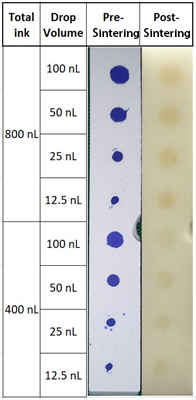
\includegraphics[width=0.38\textwidth]{grafiken/DropSize.jpg}
	\caption{Effect of the drop size on the spot area}
	\label{fig:DropSize}
\end{figure} 
A larger drop size results in shorter print duration. However they also tend to expand the spot area more compared to the smaller drops as you can see, which is bad for the resolution.The graphs show the ink intensity along the red lines and the spreading of the ink in lateral direction for each drop volume. 12.5 and 25 nL drops result in a similar spot diameter but the spots tend to get significantly larger with 50 and 100 nL Drops.
\begin{figure}[h]
	\centering
	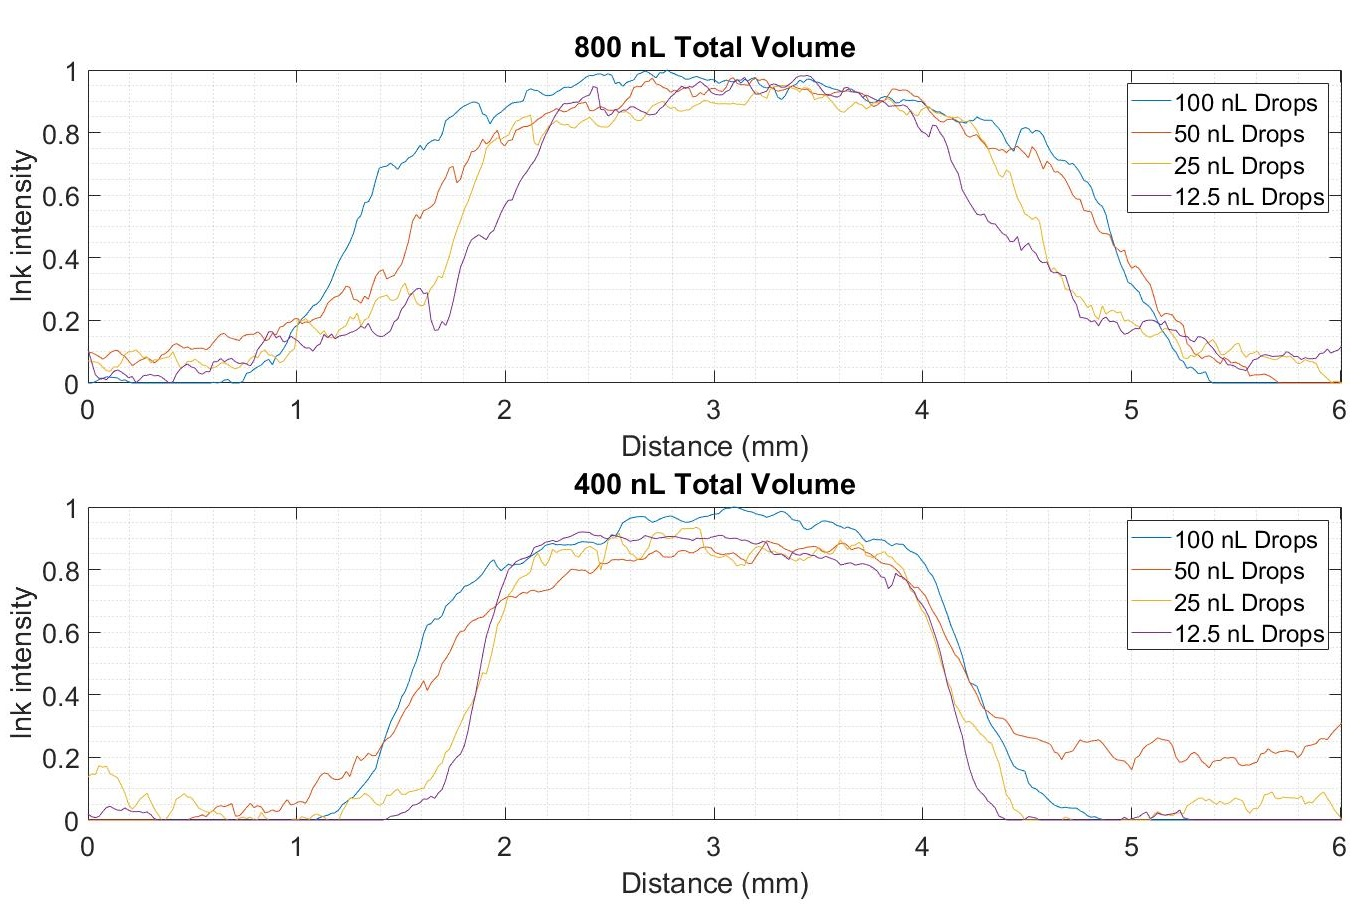
\includegraphics[width=1\textwidth]{grafiken/SpotArea.jpg}
	\caption{Comparison of the spot area results depending on the drop size}
	\label{fig:SpotArea}
\end{figure} 

\section{Point Spread Function}


The halftone tonality is greatly affected by optical dot gain a phenomena caused by the photon diffusion inside the medium. The point spread function (PSF) is one of the ways to model the optical dot gain. The derivation of an appropriate PSF is accomplished through solving the radiative transfer equation, which leads to a PSF in terms of the scattering and absorption coefficients of the medium. This PSF is then used for calculating the average diffusion distance of the photons inside medium. It is shown in the work of Rogers that the Z-sum, which can be expressed explicitly, can be estimated by $\mu^{-s}$, where $\mu$ is the fractional ink coverage and s has values between 0 and 1.  The interrelationship  between the PSF  approach and the probability approach is proven to be strong. \citep{rogers2015point}



